\documentclass[11pt,a4paper]{article}

% ---------------------------------------------------------------- packages
\usepackage[a4paper,margin=2.4cm,top=3.6cm,bottom=3cm]{geometry}
\usepackage[utf8]{inputenc}
\usepackage[T1]{fontenc}
\usepackage{lmodern}
\usepackage{amsmath,amssymb,amsthm}
\usepackage{graphicx}
\usepackage{tikz}
\usepackage{xcolor}
\usepackage{enumitem}
\usepackage{fancyhdr}
\usepackage{titlesec}
\usepackage[most]{tcolorbox}
\usepackage{listings}
\usepackage{needspace}
\usepackage[colorlinks=true,linkcolor=navy,citecolor=navy,urlcolor=navy]{hyperref}
\usepackage{booktabs}

% ---------------------------------------------------------------- UCLouvain colours (matching the course slides)
\definecolor{navy}{HTML}{00214D}
\definecolor{ucblue}{HTML}{5DB3E6}
\definecolor{ucgrey}{HTML}{8591A0}
\definecolor{ucblock}{HTML}{F2F7FB}
\definecolor{ucorange}{HTML}{E07B00}
\definecolor{ucred}{HTML}{C1272D}

% ---------------------------------------------------------------- section styling
\titleformat{\section}
  {\color{navy}\Large\bfseries}{\thesection}{0.6em}{}
\titleformat{\subsection}
  {\color{navy}\large\bfseries}{\thesubsection}{0.6em}{}
\titlespacing*{\section}{0pt}{1.4em}{0.6em}

% ---------------------------------------------------------------- "Part" headers
\newcommand{\homeworkpart}[2]{%
  \vspace{0.6em}
  \begin{tcolorbox}[colback=navy,colframe=navy,arc=0pt,boxrule=0pt,
    left=10pt,right=10pt,top=7pt,bottom=7pt]
    {\color{white}\bfseries\large Part #1 --- #2}
  \end{tcolorbox}
  \vspace{0.4em}
}

% ---------------------------------------------------------------- task / deliverable boxes
\newcounter{taskcounter}
\newtcolorbox{task}{%
  enhanced, breakable, colback=ucblock, colframe=ucblue,
  boxrule=0.8pt, arc=2pt, left=8pt, right=8pt, top=6pt, bottom=6pt,
  before skip=8pt, after skip=8pt,
  fonttitle=\bfseries\color{navy},
  title={Task \stepcounter{taskcounter}\thetaskcounter}
}
\newtcolorbox{note}{%
  enhanced, breakable, colback=white, colframe=ucgrey,
  boxrule=0.6pt, arc=1pt, left=8pt, right=8pt, top=5pt, bottom=5pt,
  before skip=6pt, after skip=6pt,
  fonttitle=\bfseries, coltitle=white, title={Note}
}

% ---------------------------------------------------------------- code listings
\lstdefinestyle{code}{
  basicstyle=\ttfamily\small,
  keywordstyle=\bfseries\color{navy},
  commentstyle=\itshape\color{ucgrey},
  stringstyle=\color{ucorange},
  numbers=left, numberstyle=\tiny\color{ucgrey}, numbersep=8pt,
  breaklines=true, breakatwhitespace=false,
  frame=single, rulecolor=\color{ucblue!60}, framesep=6pt,
  backgroundcolor=\color{ucblock},
  showstringspaces=false, tabsize=2,
  xleftmargin=1em, xrightmargin=1em,
}
\lstset{style=code}

% ---------------------------------------------------------------- header / footer (mirrors the slide deck footer)
\pagestyle{fancy}
\fancyhf{}
\renewcommand{\headrulewidth}{0pt}
\renewcommand{\footrulewidth}{0.6pt}
\fancyfoot[L]{\small\color{navy}\bfseries LMECA2170 --- Computational Geometry}
\fancyfoot[R]{\small\color{ucgrey}\thepage\ /\ \pageref{LastPage}}
\usepackage{lastpage}

% ---------------------------------------------------------------- title block
\newcommand{\ucletterhead}{%
  
\includegraphics[height=1.0cm]{figures/uclouvain.png}\\[8pt]
  {\color{navy}\rule{\linewidth}{1.6pt}}\\[10pt]
  {\color{ucblue}\rule{\linewidth}{0.8pt}}\\[14pt]
}

\begin{document}
\thispagestyle{fancy}

\ucletterhead

\begin{center}
  {\color{navy}\Huge\bfseries Computational Geometry}\\[6pt]
  {\color{navy!80}\Large Homework --- Delaunay Triangulation, Alpha Shapes \& PFEM}\\[10pt]
  {\large LMECA2170 \quad$\cdot$\quad Academic year 2026--2027}\\[8pt]
  {\color{ucgrey}Miguel De Le Court \(\cdot\) Vincent Legat \(\cdot\) Kerem Okyay \(\cdot\)
  Illy Perl \(\cdot\) Alexandre Pirot \(\cdot\). \\
  Jean-Fran\c{c}ois Remacle \(\cdot\) Felix Ruyfellaere \(\cdot\) Nathan Tihon}\\[2pt]
  {\color{ucgrey}Universit\'e catholique de Louvain}
\end{center}

\vspace{0.6em}
\noindent{\color{ucblue}\rule{\linewidth}{0.8pt}}
\vspace{0.8em}

\noindent
The project framework is available in the Git repository:\\
\url{https://git.immc.ucl.ac.be/tihonn/lmeca2170-project}

\begin{center}
  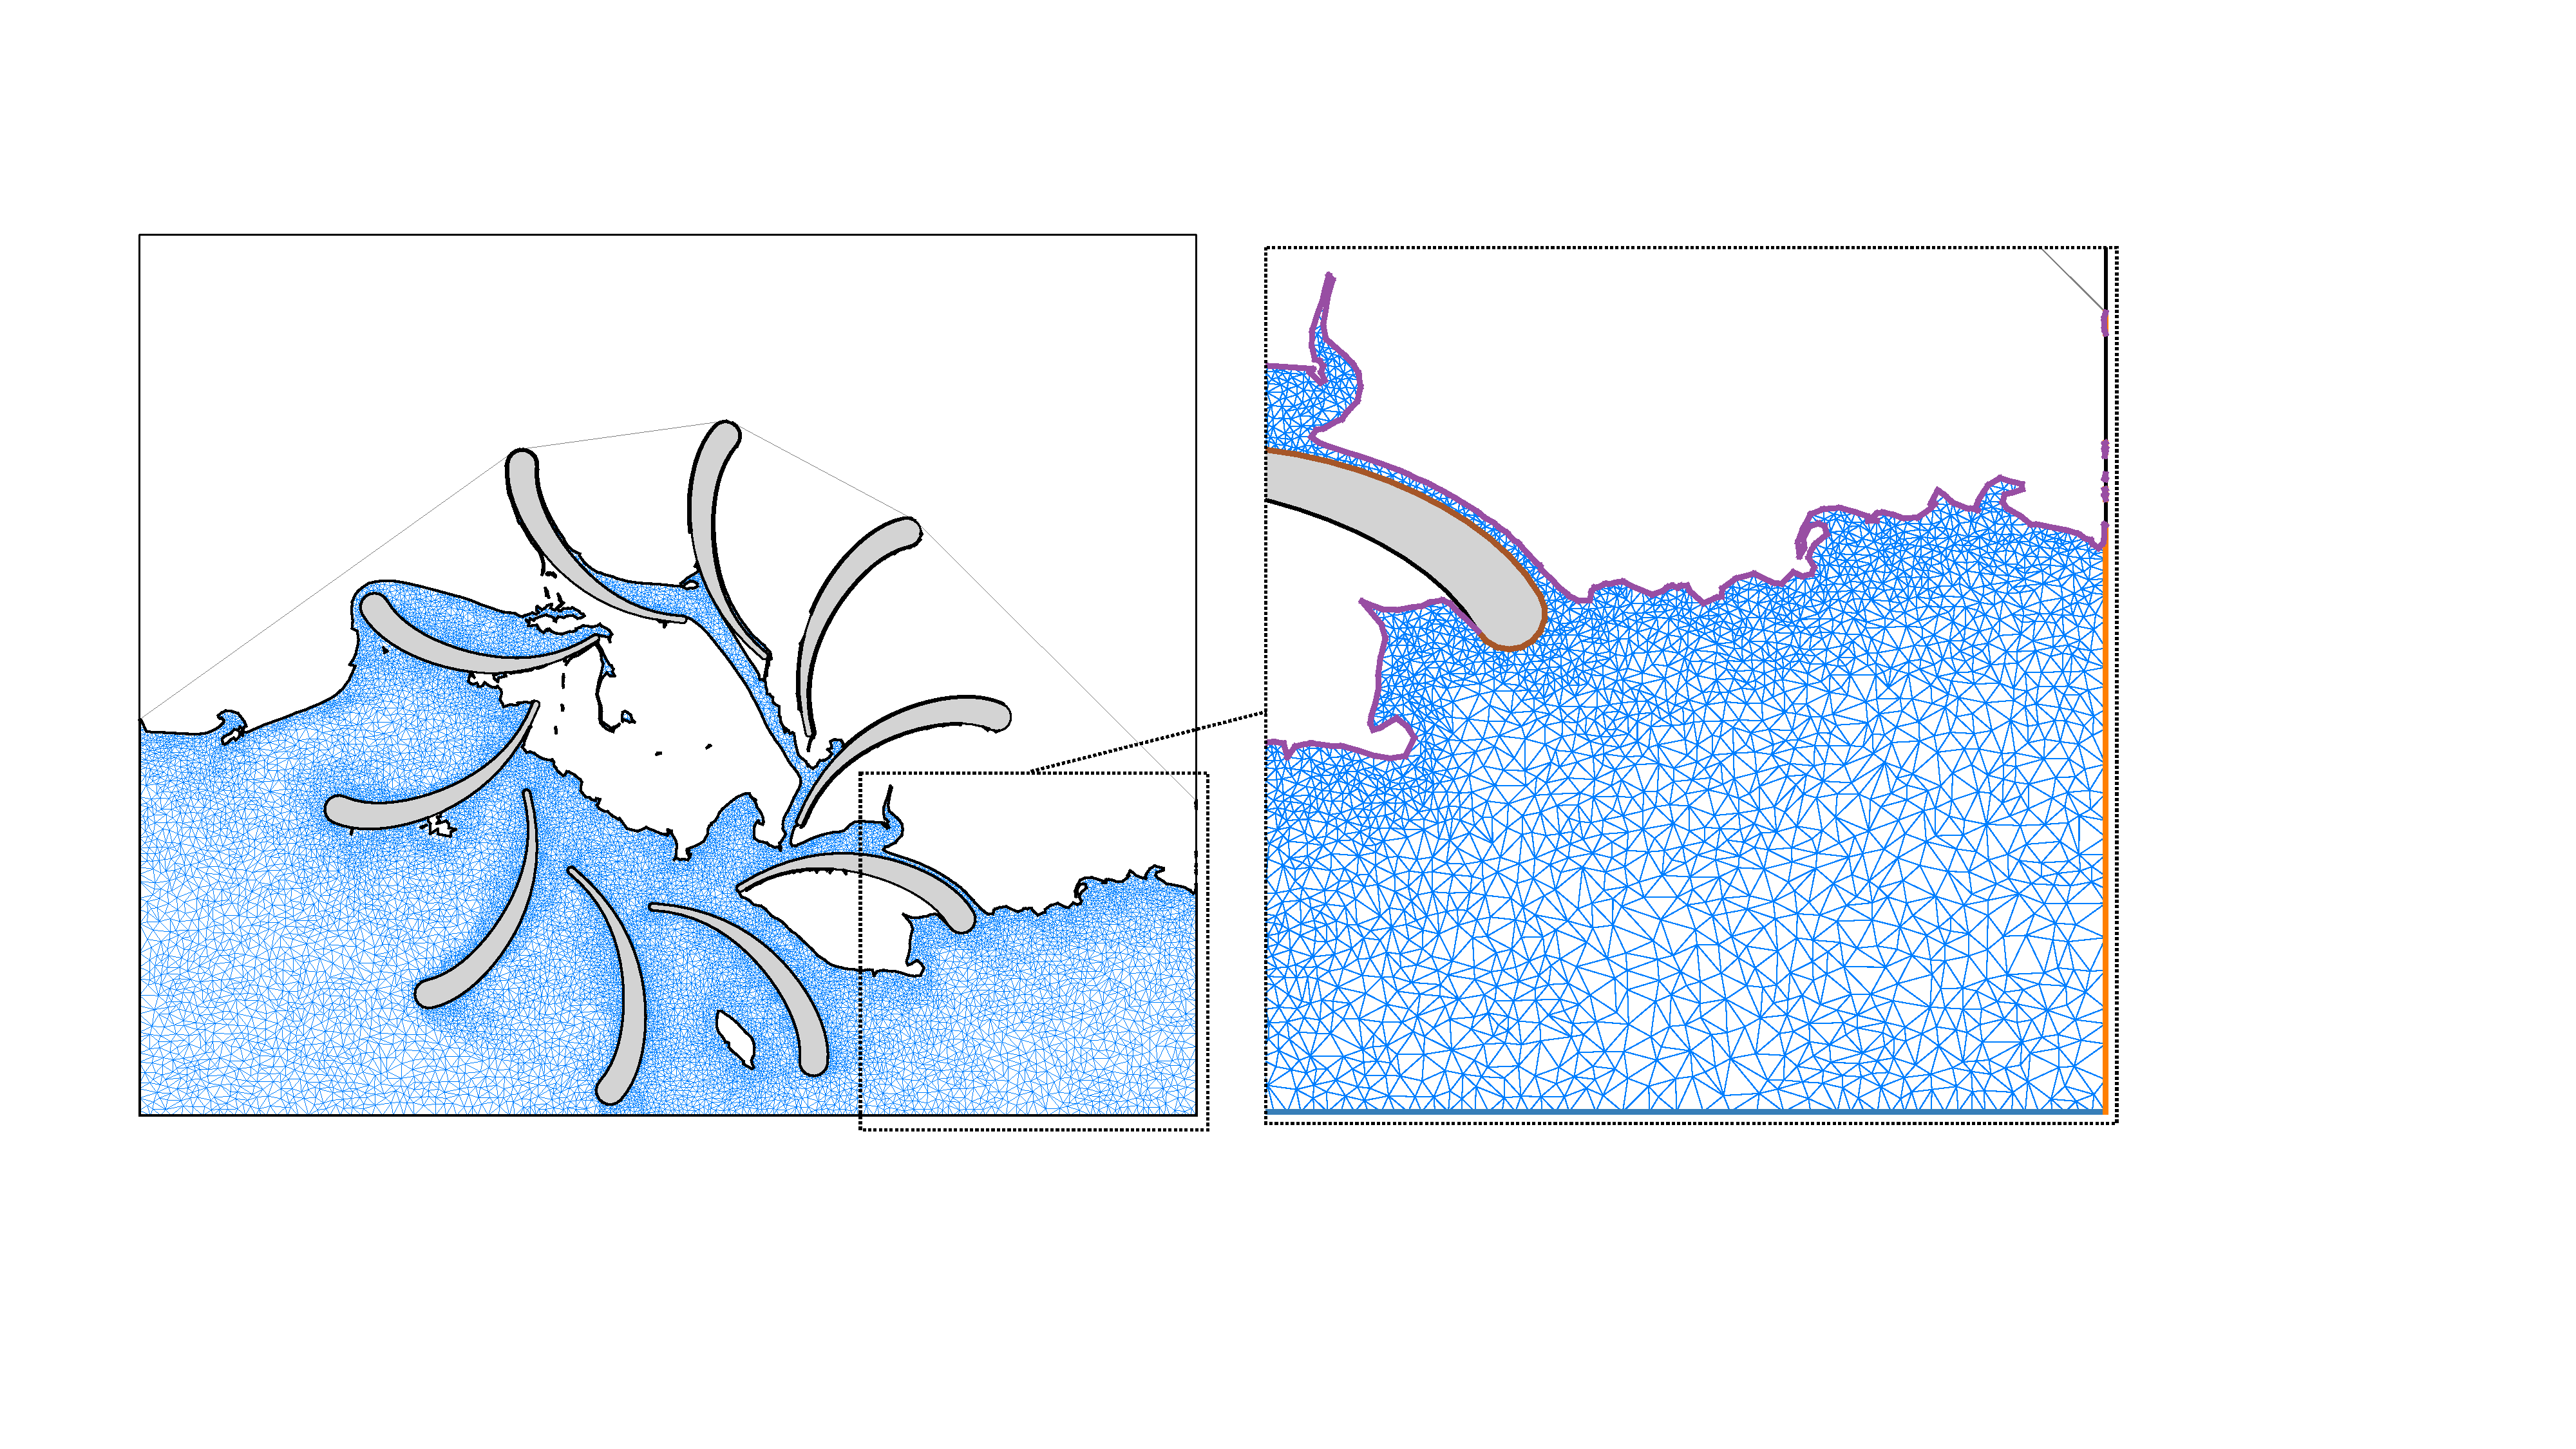
\includegraphics[width=\linewidth]{figures/wheel_illus_boundaries.pdf}
\end{center}

\noindent
This homework has three parts, each building directly on the previous one. In
\textbf{Part~1} you implement, entirely from scratch, an incremental Delaunay
triangulation on top of a half-edge data structure, and filter it into an
\emph{alpha shape}. In \textbf{Part~2} you improve that alpha shape by
inserting Steiner points with \textbf{Chew's algorithm}, reusing the exact
same insertion routine you wrote in Part~1. In \textbf{Part~3} you implement
 a \textbf{spatial search structure} for nearest-edge queries and collision
detection. Finally, you assemble everything into a \textbf{PFEM} (Particle
Finite Element Method) time-stepping loop for free-surface flows. At every
time step, the alpha shape tracks the moving fluid domain, mesh refinement
maintains mesh quality, and the search structure identifies contact with
solid walls and detects particle displacements crossing them.

\begin{note}
Read the whole statement once before starting to code: the three parts share
data structures and routines, and the way you design Part~1 will determine
how painless (or painful) Parts~2 and~3 turn out to be.
\end{note}

% ======================================================================
\homeworkpart{1}{From a Point Cloud to an Alpha Shape}
% ======================================================================

Let $S=\{p_1,\dots,p_n\}\subset\mathbb{R}^2$ be a cloud of $n$ points. The
goal of Part~1 is to compute the Delaunay triangulation $DT(S)$
incrementally, using a \textbf{half-edge} mesh data structure that you
implement yourself, and then to filter $DT(S)$ into an \textbf{alpha shape}:
a subset of the triangles that approximates the ``shape'' formed by the
points, rather than just their convex hull.

\subsection*{1.1 --- The half-edge data structure}

You are free to use any half-edge (or half-edge-like) layout, but we
recommend the classic \emph{triangle-based} scheme, since it is the
simplest one to keep synchronized while triangles are created and destroyed:

\begin{itemize}[leftmargin=1.4em]
  \item Triangles are stored as a flat array \lstinline{triangles[3*nt]}: the
    three vertex indices of triangle $t$ are
    \lstinline{triangles[3t]}, \lstinline{triangles[3t+1]}, \lstinline{triangles[3t+2]},
    listed \textbf{counter-clockwise}.
  \item Each triangle $t$ owns exactly 3 half-edges, indexed $3t,3t+1,3t+2$.
    Half-edge $3t+k$ goes from vertex \lstinline{triangles[3t+k]} to vertex
    \lstinline{triangles[3t+(k+1)%3]}.
  \item \lstinline{next(he)} needs no storage: it is simply
    \lstinline{3*(he/3) + (he+1)%3}.
  \item One array \lstinline{opposite[3*nt]} stores, for every half-edge, the
    index of its \textbf{twin} (the half-edge of the neighbouring triangle
    that runs along the same edge in the opposite direction), or $-1$ if the
    edge is on the boundary.
\end{itemize}

\begin{center}
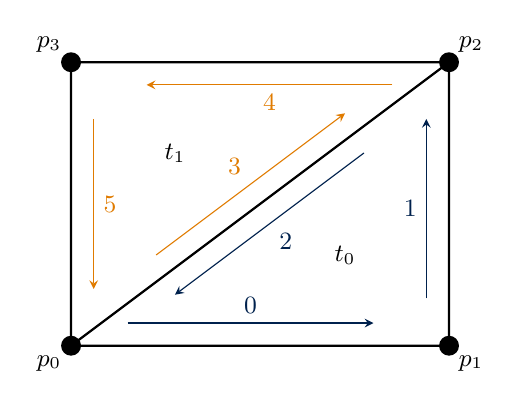
\begin{tikzpicture}[scale=2.4,>=stealth,font=\small]
  \coordinate (A) at (0,0); \coordinate (B) at (2,0);
  \coordinate (C) at (2,1.5); \coordinate (D) at (0,1.5);
  \draw[thick] (A)--(B)--(C)--(D)--cycle (A)--(C);
  \foreach \P/\n/\pos in {A/0/below left,B/1/below right,C/2/above right,D/3/above left}
    \fill (\P) circle (1.5pt) node[\pos] {$p_\n$};
  \node at (1.45,.48) {$t_0$}; \node at (.55,1.02) {$t_1$};
  \draw[->,navy] (.3,.12)--(1.6,.12) node[midway,above] {0};
  \draw[->,navy] (1.88,.25)--(1.88,1.2) node[midway,left] {1};
  \draw[->,navy] (1.55,1.02)--(.55,.27) node[midway,below right] {2};
  \draw[->,ucorange] (.45,.48)--(1.45,1.23) node[midway,above left] {3};
  \draw[->,ucorange] (1.7,1.38)--(.4,1.38) node[midway,below] {4};
  \draw[->,ucorange] (.12,1.2)--(.12,.3) node[midway,right] {5};
\end{tikzpicture}
\qquad
\begin{tabular}{c|rrr|rrr}
\toprule
Half-edge & 0 & 1 & 2 & 3 & 4 & 5 \\
\midrule
\texttt{triangles} & 0 & 1 & 2 & 0 & 2 & 3 \\
\texttt{opposite} & $-1$ & $-1$ & 3 & 2 & $-1$ & $-1$ \\
\bottomrule
\end{tabular}
\end{center}
The arrows show half-edge indices; only half-edges 2 and 3 are twins.
The four outer half-edges have no opposite in this finite mesh.

This representation is compact, cache-friendly, and --- crucially for this
homework --- \emph{local}: inserting a point only touches the half-edges of
the triangles being removed and created, never the whole mesh.

\needspace{7\baselineskip}
\begin{task}\label{tsk:halfedge}
Implement the half-edge structure above (or an equivalent one of your
choice) together with the elementary queries you will need: the two
triangles sharing an edge, the three neighbours of a triangle, and the
vertices of a triangle in CCW order.
\end{task}

\subsection*{1.2 --- Bootstrapping: one point at infinity}

Use a single \textbf{symbolic vertex at infinity} $q_\infty$, with no finite
coordinates. Start from three non-collinear input points $p_a,p_b,p_c$ in
counter-clockwise order. Create their finite triangle and the three
\emph{ghost triangles}
\[
 (p_b,p_a,q_\infty),\qquad (p_c,p_b,q_\infty),\qquad
 (p_a,p_c,q_\infty).
\]
Connect all twins, including the edges incident to $q_\infty$. A ghost
triangle represents the exterior half-plane to the left of its oriented
finite edge. Thus its finite edge is opposite to the corresponding edge
of the finite convex hull. Always store $q_\infty$ in the \textbf{third slot}
of a ghost triangle, using a cyclic permutation and updating half-edge
indices consistently. Never pass this symbolic index to coordinate-based
arithmetic.

For a finite point $D$, only two cavity-predicate cases are needed:
\begin{itemize}[leftmargin=1.4em]
  \item \textbf{Finite triangle $(A,B,C)$}, listed CCW: use the usual
    robust \lstinline{incircle(A,B,C,D)} predicate.
  \item \textbf{Ghost triangle $(A,B,q_\infty)$}: use
    \[
      \operatorname{incircle}(A,B,q_\infty,D)>0
      \quad\Longleftrightarrow\quad
      \operatorname{orient2d}(A,B,D)>0.
    \]
    A positive sign means that $D$ lies outside the current convex hull,
    on the exterior side represented by this ghost triangle.
\end{itemize}
Handle zero predicates consistently. Detect duplicate points and the
all-collinear input case explicitly; the latter has no two-dimensional
triangulation. This construction avoids a large finite super-triangle and
requires no arbitrary ``far away'' coordinates.

\subsection*{1.3 --- Insertion order: sorting indices along a Hilbert curve}

A Hilbert space-filling curve can improve spatial locality during point
insertion. Compute a Hilbert key for each point, then sort an array of
\textbf{point indices}, leaving coordinates and nodal fields in their
original order. For example,
\begin{center}
\begin{tabular}{lrrrr}
\toprule
Point index & 0 & 1 & 2 & 3 \\
Hilbert key & 8 & 56 & 34 & 1 \\
\midrule
Insertion order & 3 & 0 & 2 & 1 \\
\bottomrule
\end{tabular}
\end{center}
Skip the three points already used for bootstrapping. Consecutive
insertions often lie near one another, which helps the point-location walk
in practice; no constant-time guarantee is assumed.

\begin{task}
Implement an insertion permutation based on Hilbert keys at a fixed
recursion depth. Keep point identifiers and the associated physical fields
unchanged. Compare the walking cost with an unsorted insertion order.
\end{task}

\subsection*{1.4 --- Locating the point: a stochastic visibility walk}

For every point $p$ (in Hilbert order), first find the triangle $T_0$ that
contains it, starting the walk from the triangle in which the
\emph{previous} point was inserted:

\needspace{12\baselineskip}
\begin{lstlisting}[style=code,caption={Stochastic visibility walk},captionpos=b]
T <- last triangle used
loop:
  if T is a ghost triangle (a,b,infinity):
      if orient2d(a,b,p) > 0: T0 <- T; stop
      T <- finite neighbour across (a,b)
      continue the loop
  let (u,v,w) be the vertices of finite T, CCW
  test the 3 edges (u,v),(v,w),(w,u) of T in a *random* order
  for the first edge (a,b) such that orient2d(a,b,p) < 0:
      cross into the triangle across (a,b);  T <- that triangle
      continue the loop
  # no edge tested negative: p is inside T
  T0 <- T;  stop
\end{lstlisting}

The predicate \lstinline{orient2d(a,b,p)} returns (twice) the signed area of
$abp$: negative means $p$ lies to the right of the oriented edge
$a\!\to\!b$, i.e.\ outside the triangle on that side.

\begin{note}
Randomizing the order in which the 3 edges are tested at every step is not
cosmetic: on a triangulation that is not Delaunay (which can happen
transiently, or if you experiment with non-Delaunay meshes), a
\emph{deterministic} edge order can make the walk cycle forever. The
randomized version almost surely terminates. On a genuine Delaunay
triangulation the walk always terminates, deterministic or not --- but get
into the habit of randomizing, it costs nothing and removes an entire class
of bugs.
\end{note}

\subsection*{1.5 --- Building the Delaunay cavity}

Starting from $T_0$, grow the \textbf{cavity} of $p$ breadth-first: a
triangle belongs to the cavity if and only if $p$ lies strictly inside its
circumcircle (the \lstinline{incircle} predicate).

\needspace{12\baselineskip}
\begin{lstlisting}[style=code,caption={Cavity computation (BFS)},captionpos=b]
cavity <- {T0};  Q <- [T0]
while Q is not empty:
   T <- Q.pop_front()
   for each neighbour T' of T, across shared edge e:
       if T' not in cavity and incircle(T', p) > 0:
           cavity <- cavity + {T'}
           Q.push(T')
# Extract the boundary only after the cavity is complete:
boundary <- all half-edges in cavity whose twin is outside cavity
order boundary by following its connected edge loop
\end{lstlisting}

At the end, \lstinline{boundary} is the ordered set of edges bounding the
star-shaped hole left by removing every triangle of \lstinline{cavity}.

\subsection*{1.6 --- Retriangulating the cavity}

Delete every triangle of \lstinline{cavity} and create one new triangle
$(a,b,p)$ for every boundary edge $(a,b)$, connecting $p$ to the whole
boundary loop (a \emph{fan}). This is the step where the half-edge structure
must be updated \textbf{locally}:

\begin{itemize}[leftmargin=1.4em]
  \item for each new triangle $(a,b,p)$, set the twin of its edge $(a,b)$ to
    whatever triangle used to be on the other side of that boundary edge
    (unchanged, since that neighbour was \emph{not} in the cavity);
  \item set the twins of the two new internal edges ($b\!\to\!p$ and
    $p\!\to\!a$) to their counterparts in the two adjacent new fan triangles.
\end{itemize}

Update the surviving neighbours' twin references to point to the new
half-edges. No other half-edge needs to be touched. If a new triangle
contains $q_\infty$, cyclically rotate its vertices to keep that vertex last.

\begin{task}\label{tsk:bowyerwatson}
Implement the full incremental Bowyer--Watson loop: one-point-at-infinity
bootstrap, index-based Hilbert insertion, visibility walk, cavity and
retriangulation. Once all input points have been inserted, discard the
ghost triangles and set exposed twin references to $-1$. The remaining
finite mesh is $DT(S)$.
\end{task}

\subsection*{1.7 --- Filtering into an alpha shape}

An \textbf{alpha shape} of parameter $\alpha>0$ is obtained by removing,
from $DT(S)$, every triangle whose circumradius exceeds $\alpha$. Loosely,
$\alpha$ acts as a probe radius: triangles that could only exist because
Delaunay triangulates the \emph{convex hull} of $S$ --- bridging concavities
or holes with large, thin triangles --- have a large circumradius and
disappear, while the triangles that genuinely reflect the local density of
$S$ survive.

\begin{task}
Compute the circumradius of every triangle of $DT(S)$ and remove those
exceeding a user-supplied $\alpha$. Test on a point cloud shaped like a
non-convex outline (e.g.\ a letter, an annulus, or two point clusters joined
by a thin bridge) and check that the result visually matches the cloud's
shape for a reasonable range of $\alpha$, and degenerates back towards the
convex hull as $\alpha\to\infty$.
\end{task}

\paragraph{A single global $\alpha$ is not always enough.} A value large
enough to retain a sparsely sampled region may bridge gaps in a densely
sampled region; a smaller value can remove valid triangles in the sparse
region. Assign a local size $\alpha_i>0$ to each node, and derive a threshold
for each triangle $T=(i,j,k)$ from its \emph{nodal} values:
\[
 \alpha_T^{\mathrm{avg}}=\frac{\alpha_i+\alpha_j+\alpha_k}{3},\qquad
 \alpha_T^{\min}=\min(\alpha_i,\alpha_j,\alpha_k),\qquad
 \alpha_T^{\max}=\max(\alpha_i,\alpha_j,\alpha_k).
\]
Retain $T$ when its circumradius is at most the chosen $\alpha_T$.
This spatially varying filter generalizes the constant-radius construction.
Do not sample the size field at the circumcenter: that requires an extra
query and can be misleading, for example when many triangles have the same
circumcenter despite different local sampling densities.

\begin{task}
Compare the average, minimum and maximum nodal thresholds on a point cloud
with non-uniform density. Discuss which triangles each choice retains and
how it affects holes and thin features. Start from an analytic nodal size
field; other aggregation rules may also be investigated and justified.
\end{task}

\begin{note}
Export your triangulation to Gmsh's \texttt{.pos} format (or any format you
can visualize) at every stage --- after Bowyer--Watson and after alpha
filtering. Kerem's OpenGL renderer is another option, including for
interactive inspection, when made available --- so you can \emph{see} bugs instead of guessing at them.
\end{note}

% ======================================================================
\homeworkpart{2}{Improving the Alpha Shape --- Chew's Algorithm}
% ======================================================================

Simply deleting large-circumradius triangles can leave behind a shape with a
jagged, uneven boundary: a triangle can be thin and skinny yet still have a
circumradius just under $\alpha$, so it survives the filter even though it
poorly represents the local shape. \textbf{L.~Paul Chew's algorithm}
(1989/1993) improves this by \emph{adding} well-chosen points to the
triangulation rather than only removing triangles --- and it reuses the point-insertion machinery of Part~1, with
additional care to preserve the extracted boundary.

\subsection*{2.1 --- The idea}

Refine the domain \emph{after} extracting its alpha shape. Preserve its
boundary segments and holes during insertion. A triangle $T$ is
\textbf{bad} if its circumradius-to-shortest-edge ratio exceeds a chosen
bound $\rho$, or if it exceeds the local target size. Since
$R_T/\ell_{\min,T}=1/(2\sin\theta_{\min,T})$, a bound $\rho=1$ corresponds
to a minimum angle of $30^\circ$ for triangles satisfying it.

\begin{lstlisting}[style=code,caption={Boundary-preserving refinement},captionpos=b]
repeat:
    find a bad triangle T (quality or local size criterion)
    if none exists: stop
    c <- circumcenter(T)
    if c is admissible and encroaches on no protected segment:
        insert c; update the local mesh and nodal size values
    else:
        split the relevant protected boundary segment
        or record T as unresolved under your boundary policy
    stop if the iteration or point-count limit is reached
\end{lstlisting}

The circumcenter is the centre of an empty circle, which motivates its use
as a candidate Steiner point. Reuse the insertion machinery of Part~1, but
adapt it to respect the protected boundary: it must not create triangles
across holes or outside the retained domain. Splitting a protected segment
must preserve its geometry and update both connectivity and boundary data.

\subsection*{2.2 --- Refinement order and stopping criteria}

Use the sequence \textbf{triangulation $\to$ alpha-shape extraction $\to$
mesh refinement}. A second alpha-shape extraction is not required: the
refinement step is intended to improve the mesh of the already selected
domain. Refining the whole convex-hull triangulation \emph{before}
filtering can populate holes with Steiner points and change the shape
subsequently detected by the filter.

\begin{note}
Preserving the domain during refinement does not prove that filtering the
new triangulation would return the same alpha shape, especially with
spatially varying nodal thresholds. Explain the assumptions needed for
such a claim. Likewise, termination guarantees for established refinement
algorithms depend on their boundary rules and geometric assumptions;
they do not automatically apply to every simplified implementation.
\end{note}

\begin{task}\label{tsk:chew}
Implement a Chew-inspired refinement loop on the extracted alpha shape,
with an explicit policy for circumcenters outside the domain and for
encroached boundary segments. Explain how holes are preserved. Set iteration
and point-count limits, report unresolved bad triangles and track quality
throughout refinement; the number of bad triangles need not decrease
monotonically. Explain why refinement before filtering can change the
reconstructed domain. Do not re-apply the alpha filter as a routine second
step.
\end{task}

\begin{task}
Compare, on the same test point cloud(s) as Part~1, the alpha shape before
and after Chew refinement: report the number of triangles, the minimum
angle, and the number of triangles that fail the quality bound $\rho$, in
each case.
\end{task}

% ======================================================================
\homeworkpart{3}{Spatial Search Structures and PFEM Integration}
% ======================================================================

Implement a spatial search structure, such as a \textbf{quadtree}, on the
fixed solid boundary segments. These segments are stored independently of
the fluid particles and mesh. Finally, use the structure in a
\textbf{Particle Finite Element Method} (PFEM) loop: the fluid particles
move with the velocity field, and Parts~1 and~2 rebuild their domain and
refine its mesh at each step.

\subsection*{3.1 --- Nearest-edge queries and collision detection}

Your structure must support two queries:
\begin{itemize}[leftmargin=1.4em]
  \item \textbf{Nearest solid edge to a point.} Return the nearest segment,
    the closest point on it and the distance. Use this to distinguish wall
    contact from the free surface, with a documented distance tolerance.
  \item \textbf{First intersection with a displacement segment.} Given a
    particle's current and proposed positions, return the first solid edge
    hit and its parameter along the displacement. Shorten the displacement
    to keep the particle on the admissible side of the wall.
\end{itemize}
Store or reference every segment in all cells it intersects, or use a
bounding-box hierarchy with a documented storage rule. Prune nearest-edge
queries using distance lower bounds; checking only the point's own cell is
not sufficient. For collision queries, search all cells crossed by the
motion and select the earliest valid hit. Treat endpoint contacts,
collinear motions and particles already on a wall consistently.

\begin{task}
Implement both queries and validate them against an exhaustive scan of all
solid edges. Measure query cost as the number of edges and particles grows.
Document your subdivision rule, contact tolerance and collision policy.
\end{task}

\subsection*{3.2 --- The provided solver and the PFEM loop}

The fluid solver is provided; you do not need to implement its finite
element formulation. The following C interface is a \textbf{provisional
contract}, to be confirmed with the supplied implementation. Python users
will need the corresponding binding or wrapper.

\begin{lstlisting}[style=code,language=C,caption={Provisional solver interface},captionpos=b]
#include <stdint.h>
typedef enum {
    BULK = 0, FREE_SURFACE = 1, WALL = 2
} node_type_et;

typedef struct {
    int success;
} solver_status_st;

typedef struct {
    double density;       // rho
    double viscosity;     // nu; convention to be confirmed
    double gravity[2];
    double dt;
} physical_props_st;

solver_status_st solve_navier_stokes(
    double const *nodes, uint32_t nnodes,
    uint32_t const *elems, uint32_t nelems,
    node_type_et const *node_type,
    uint32_t const *bnd_edges, uint32_t n_bnd_edges,
    physical_props_st const *props, double *uvp);
\end{lstlisting}

Coordinates are interleaved $(x_0,y_0,x_1,y_1,\ldots)$, with length
$2n_{\mathrm{nodes}}$; elements contain $3n_{\mathrm{elems}}$ vertex indices
in CCW order. The array \texttt{node\_type} contains one classification per
node. The array \texttt{bnd\_edges} contains $2n_{\mathrm{bnd\_edges}}$
indices describing the \emph{current fluid-mesh boundary}, not the independent
solid-wall geometry. The caller allocates \texttt{uvp}, of length
$3n_{\mathrm{nodes}}$. It stores the interleaved input/output values
\[
  (u_0,v_0,p_0,u_1,v_1,p_1,\ldots).
\] Check the returned solver status before moving particles.

In this provisional contract, bulk nodes have velocity and pressure degrees
of freedom; free-surface nodes use the prescribed pressure $p=0$; wall
nodes impose no slip, $u=v=0$. The solver handles pressure consistently
with its formulation; a wall classification does not prescribe $p=0$.

\needspace{30\baselineskip}
\begin{lstlisting}[style=code,caption={PFEM driver},captionpos=b]
read/construct the fixed solid boundary segments
build their quadtree once
initialize fluid positions, nodal sizes and (u,v,p)

for each time step:
    triangulate the fluid points; extract the alpha shape
    refine the retained domain, preserving its boundaries
    transfer fields and sizes to any new nodes
    bnd_edges <- fluid-mesh edges with no opposite
    node_type <- BULK for every node
    for each node belonging to bnd_edges:
        query nearest solid edge
        classify as WALL if within contact tolerance
        otherwise classify as FREE_SURFACE
    choose dt using the mesh size and velocity
    status <- solve_navier_stokes(...)
    if not status.success: stop and report the failure

    for each fluid node i:
        displacement <- dt * (u[i],v[i])
        query first wall hit along this displacement
        shorten displacement if needed to prevent crossing
        coord[i] <- coord[i] + displacement
    save/plot the current state
\end{lstlisting}

\subsection*{3.3 --- Practical points}

\begin{itemize}[leftmargin=1.4em]
  \item \textbf{Independent walls.} Solid boundary segments do not move,
    are not fluid elements and need not be triangulated. They provide the
    geometry for contact and crossing queries. Fluid nodes in contact are
    classified separately and receive the solver's wall condition.
  \item \textbf{Mesh-size field.} Start with a constant target spacing
    $h_i$ and take $\alpha_i=c h_i$ with a documented factor $c>0$.
    As an extension, try a bounded size field based on distance to the free
    surface, the velocity gradient or vorticity. Explain the physical or
    geometric features targeted by your choice.
  \item \textbf{Field transfer.} Interpolate velocity, pressure and nodal
    size values to Steiner points. If you remove points, update all
    associated fields and indices consistently. Document this transfer;
    it is essential to keep remeshing and the solver compatible.
  \item \textbf{Time step.} For this homework, use the displacement-based
    CFL guideline
    \[
      U_{\max}\frac{\Delta t}{h_{\min}}\leq\beta,
      \qquad 0<\beta<1,
    \]
    where $U_{\max}=\max_i\sqrt{u_i^2+v_i^2}$ and $h_{\min}$ is the minimum
    triangle altitude of the current mesh. State your choice of $\beta$
    and impose a maximum time step when $U_{\max}=0$. This geometric
    guideline does not replace other restrictions of the provided solver;
    collision queries are still required after the velocity update.
\end{itemize}

\begin{task}
Assemble the driver around \lstinline{solve_navier_stokes}, reusing
Parts~1 and~2 and your spatial search structure. Document field transfer,
node classification and handling of wall collisions.
\end{task}

\begin{task}
Demonstrate the implementation on a \textbf{dam-break} test: a rectangular
column of fluid, initially at rest, collapses under gravity in a rigid
tank. Provide snapshots or a short video of the evolving mesh and free
surface, and check that particles do not cross the solid walls.
\end{task}



% ======================================================================
\section*{Practical Information}
% ======================================================================

\begin{itemize}[leftmargin=1.4em]
  \item \textbf{Language.} You may use \textbf{C, C++ or Python}.
    The repo contains a skeleton of the project in C because Nathan thinks
    you should do it in C. But he knows C can be scary so he's included a
    tutorial on how to call C functions from Python in
    \path{docs/python-binding-example/}. This way you can use Python for
    the high-level logic and still implement the performance-critical
    parts in C !
  \item \textbf{Predicates and sorting.} Using an existing, well-tested
    implementation of \lstinline{orient2d} and \lstinline{incircle} (e.g.\
    Shewchuk's robust predicates) is clearly \textbf{allowed} --- Part~1 is
    about the triangulation algorithm and its data structure, not about
    re-deriving exact arithmetic. Likewise for the Hilbert sort: you may use
    an existing implementation, e.g.\
    \url{https://git.immc.ucl.ac.be/hextreme/HXTSort}.
  \item \textbf{Deliverables.} Your source code (buildable from a clean
    checkout, with a short \texttt{README}), together with a short report
    (max.\ 4 pages) describing your data structures, any design choices left
    open in the statement, and the results asked for in Parts~1--3.
    Four pages is a maximum, not a target: focus on your design choices,
    tests and results rather than repeating the lectures or this statement.
  \item \textbf{Visualization.} Choice of weapons: there are plenty of
    reasonable options, and you are free to pick whichever suits you. Both
    \textbf{ParaView} and \textbf{Gmsh} are well suited to this kind of
    work --- e.g.\ export your triangulations in Gmsh's \texttt{.pos} format
    so that you can inspect your own results at every stage of development.
    Kerem's OpenGL renderer is also an option for visualization and
    interactivity when made available.
  \item \textbf{Deadline.} \emph{[to be announced on \href{https://perso.uclouvain.be/vincent.legat/zouLab/meca2170.php}{zouLab web site}]}.
  \item \textbf{Academic integrity.} Work in \textbf{groups of two}. You may
    discuss ideas with classmates, but the submitted code and report must
    reflect your group's work and understanding.
  \item \textbf{Use of AI.} You may use AI to help you understand and
    implement the tasks. Both members must understand the submitted code
    and be able to explain its design and limitations. A solution you
    understand, even with flaws you can explain, is preferable to a
    functioning program you cannot explain. The purpose of this project
    is to learn the course material.
\end{itemize}

\end{document}
